\section{Analysis}
\label{sec:analysis}



\begin{figure}[t!]
\centering

\subfloat{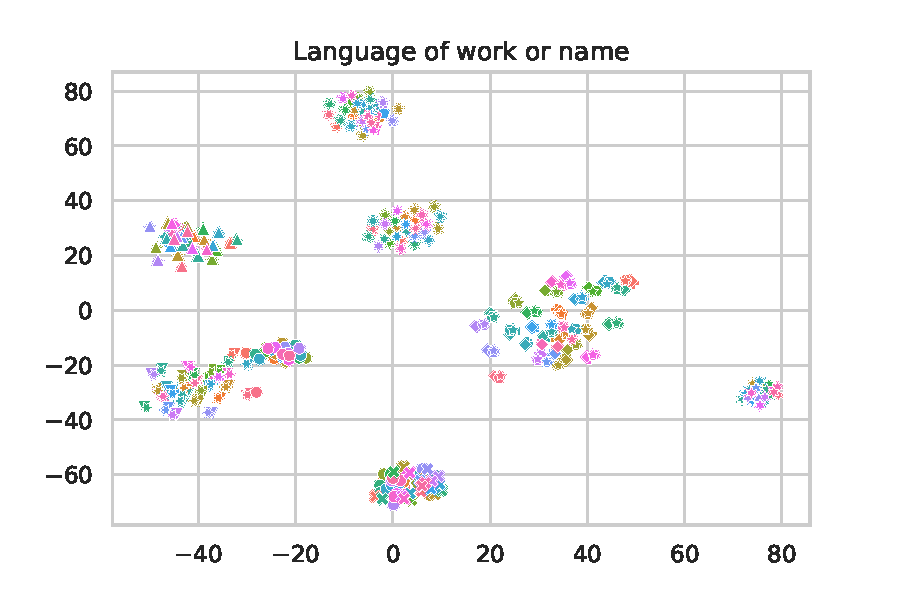
\includegraphics[width=1.\columnwidth]{figures/P407_emb.pdf}}\\
%   \hfill
\subfloat{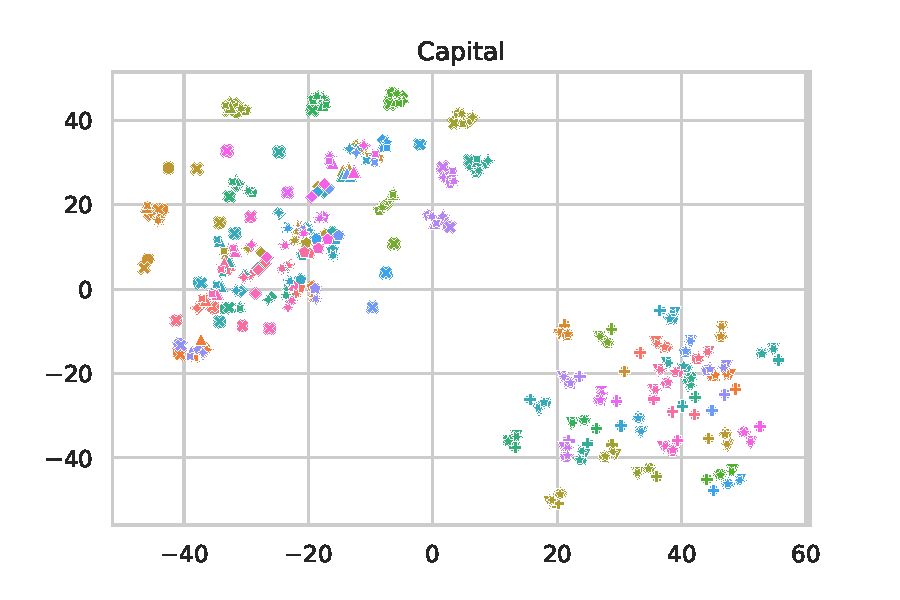
\includegraphics[width=1.\columnwidth]{figures/P36_emb.pdf}}
% \\


\caption{t-SNE plots for encoded patterns from the ``Language of work or name'' and ``Capital'' relations. Points of the same color represents same subject, Points of the same shape represents same pattern. A consistent representation should cluster based on subjects (colors) rather than patterns (shapes).}
\label{fig:tsne-emb}

\end{figure}

To provide additional insights on the way models operate on the patterns with the masked tokens they need to predict, we inspect their representations after encoding the cloze-style patterns.
We encode the patterns, populated with 50 random subjects along with the masked token, and inspect the final layer in the masked token index for all the paraphrases of multiple relations.
Then, we use t-SNE \cite{tsne} and present the results in Figure \ref{fig:tsne-emb}.
Each point represents a specific tuple, and are colored by the subjects, and the shape stands for the pattern.
A good representation would cluster the vectors together based on the subject, as then the predictions would more likely to be consistent. However, clusters based on patterns would suggest a worse encoding, since the subjects, which are of great importance in these paraphrases, are less taken into account in the representation.

We display the t-SNE figures for two relations, \textit{Language  of work or name} and \textit{Capital} in Figure \ref{fig:tsne-emb}.
It is clear that the first figure clusters mainly on the patterns, whereas the second figure clusters mainly on the subjects. These results are also consistent with the performance of these relations: @@\% and @@\%, which suggests a better representation for the later.
Additionally, we also perform clustering for the representations,\footnote{Using the KMeans algorithm.} once with the number of subjects and once with the number patterns, given as an oracle, hoping to fit the subjects or patterns clusters. Then, we calculate the v-measure metric for measuring the purity of each cluster.
A higher score on the subject-based would suggest a representation that better fits the purpose of a KB.
The v-measure results for these patterns are presented in Table \ref{tab:vmeasure-small}.
As expected, the pattern-based clustering is better for the \textit{language of work or name} relation is higher than the subject-based, and vice versa for the \textit{capital} relation.
The full clustering measures for all relations are reported in the Appendix.
\ar{Can we report correlation with performance for all relations here? Or say that in general we observe this trend?}
\begin{table}[t]
% \small
    \centering
% \resizebox{1\textwidth}{!}{%
\begin{tabular}{lrr}
\toprule
                                          Pattern &  pattern &  subject \\
\midrule
     language of work or name &            0.72 &            0.24 \\
                      capital &            0.41 &            0.62 \\
\bottomrule
\end{tabular}

% }
    \caption{V-measure clustering performance for the two relations. Reporting the results for clustering based on the pattern, and based on the subjects.}
    \label{tab:vmeasure-small}
\end{table}
